\documentclass[12pt]{article}
\title{Project Report \#1}
\author{Andre Sealy, Federica Malamisura, Swapnil Pant}
\usepackage{amsmath, amsfonts, amssymb, amsthm,}
\usepackage{tikz}
\usetikzlibrary{matrix,positioning}
\tikzset{bullet/.style={circle,fill,inner sep=2pt}}
\usepackage{braket}
\usepackage{bbold}
\usepackage[margin=1.0in]{geometry}
\usepackage{mathtools}
\usepackage{xfrac}
\usepackage{xcolor}
\newcommand{\lam}{$\lambda$}
\usepackage{pgfplots}
\tikzset{My Style/.style={samples=100, thick}}
\usepackage{graphicx}
\usepackage{pgfplots}
\usepackage{setspace}
\usepackage{enumerate}
\usepackage{hyperref}
\usepackage{array}
\usepackage{listings}
\usepackage[official]{eurosym}
\usepackage[shortlabels]{enumitem}
\usepackage{booktabs}
\usepackage{floatrow}
\usepackage{listings}
\floatsetup[table]{capposition=top}
\usepackage{appendix}
\usepackage{xcolor}
\hypersetup{
colorlinks,
linkcolor={red!50!black},
citecolor={blue!50!black},
urlcolor={blue!80!black}
}

\definecolor{codegreen}{rgb}{0,0.6,0}
\definecolor{codegray}{rgb}{0.5,0.5,0.5}
\definecolor{codepurple}{rgb}{0.58,0,0.82}
\definecolor{backcolour}{rgb}{0.95,0.95,0.92}

\lstdefinestyle{mystyle}{
backgroundcolor=\color{backcolour},   
commentstyle=\color{codegreen},
keywordstyle=\color{magenta},
numberstyle=\tiny\color{codegray},
stringstyle=\color{codepurple},
basicstyle=\ttfamily\footnotesize,
breakatwhitespace=false,         
breaklines=true,                 
captionpos=b,                    
keepspaces=true,                 
numbers=left,                    
numbersep=5pt,                  
showspaces=false,                
showstringspaces=false,
showtabs=false,                  
tabsize=2
}
\onehalfspacing

\lstset{style=mystyle}

\begin{document}

\maketitle

\section{Overview of the Asset and the Market}

The asset class for our time series analysis consists of equities primarily in the Technology sector. The reason for choosing the technology sector out of many industry classifications is multifaceted and involves numerous foundational considerations. First, we consider that tech stocks often have higher betas (meaning, they move with the market) on average, suggesting higher annualized volatility. Second, they are more sensitive to new information related to innovation cycles, such as new product releases, software updates, and research. Finally, we have the growth aspect, which involves the shifts in macroeconomic trends (such as interest rates), global demand, and supply chains. The border macroeconomic environment and the fundamentals make tech stocks an ideal candidate for time series analysis.

\section{Properties of the Time-Series}

In this section, we will outline foundational descriptive statistics, which involve the statistical moments and distributions of our sample securities and time series analysis.

\subsection{Descriptive statistics}
First, we outline a few sample statistics for the stocks in our sample. These statistics involves the sample mean, denoted by
\begin{equation}
	\hat{\mu}_x=\frac{1}{T}\sum_{t=1}^{T}x_t,
\end{equation}
the sample standard deviation, denoted by,
\begin{equation}
	\hat{\sigma}_x=\sqrt{\frac{1}{T-1}\sum_{t=1}^{T}\left(x_t-\hat{\mu}_2\right)^2},
\end{equation}
the sample skewness, denoted by
\begin{equation}
	\hat{S}(x)=\frac{1}{\left(T-1\right)\hat{\sigma}^3_x}\sum_{t=1}^{T}\left(x_t-\hat{\mu}_x\right)^3,
\end{equation}
and the sample kurtosis (excess kurtosis), denoted by
\begin{equation}
	\hat{K}(x)=\frac{1}{\left(T-1\right)\hat{\sigma}^4_x}\sum_{t=1}^{T}\left(x_t-\hat{\sigma}_x\right)^4.
\end{equation}
The sample mean, $\hat{\mu}_x$ represents the daily average simple (or log) returns, where $T$ are the number of days in the sample. The sample standard deviation, denoted by $\hat{\sigma}_x$, represents the daily realized volatility, the universal risk measurement. Table (\ref{tab:descriptive}) shows the descriptive statistics of the tech stocks in our sample of the daily sample returns. The start date of our analysis is January 3rd, 2007, which gives us a time interval of roughly 18 years. In addition to the sample mean, standard deviation, skewness, and excess kurtosis, we have also decided to include the minimum and maximum prices within this time period for a better perspective.
\begin{table}[ht]
	\centering
	\caption{Descriptive statistics of Tech Stocks (\textit{Daily Simple Returns \%})}
	\begin{tabular}[t]{lcccccc}
		\toprule
		Security & Mean ($\hat{\mu}_x$) & Std Dev ($\hat{\sigma}_x$) & Skewness ($\hat{S}(x)$) & Kurtosis ($\hat{K}(x)$) &Min&Max \\
		\midrule
		QCOM & 0.05 & 2.17 & 0.27 & 9.53 &-15.25&23.20 \\
		\bottomrule
	\end{tabular}\label{tab:descriptive}
\end{table}

The returns between our sample securities are roughly similar when we look at daily log returns in Table (\ref{tab:log_descriptiv}).

The sample skewness measures the asymmetry of a probability distribution around the sample mean. It helps determine whether our sample is skewed more towards one side of the distribution. If the sample skewness, $\hat{S}(x)\approx 0,$ the distribution is symmetrical. Based on skewness, QCOM, CSCO is roughly symmetrical, as the skewness is approximately 0. 
\begin{table}[ht]
	\centering
	\caption{Descriptive statistics of Tech Stocks (\textit{Daily Log Returns \%})}
	\begin{tabular}[t]{lcccccc}
		\toprule
		Security & Mean ($\hat{\mu}_x$) & Std Dev ($\hat{\sigma}_x$) & Skewness ($\hat{S}(x)$) & Kurtosis ($\hat{K}(x)$) &Min&Max \\
		\midrule
		QCOM & 0.21 & 1.06 &-1.53 & 5.03 &-16.54 &3.18 \\	
		\bottomrule
	\end{tabular}\label{tab:log_descriptiv}
\end{table}
On the hand, the sample kurtosis measures how heavy the tails of the probability distribution are, which helps assess the presence of extreme values and the frequency of their occurrence. A normal distribution has a sample kurtosis of  $\hat{K}(x)\approx 3$, which indicates a normal distribution. All of the securities in our sample have extremely high kurtosis, which is natural for equities, considering financial markets experience extreme price movements more frequently than a normal distribution would predict. Financial markets also show periods of high and low volatility; when volatility spikes, returns tend to have more extreme values.

Considering the sample skewness, AMD is much further away from 0. There is some slight positive skew QCOM. We do not have a single sample statistic that we can use to differentiate skewed versus unskewed. However, we can test for skewness using the Jarque and Bera test for normality.

The Jarque-Bera (JB) test is a statistical test used to check whether a dataset follows a normal distribution. It does this by examining the skewness and kurtosis of the dataset with the following formula:
\begin{equation}
	JB= \underbrace{\frac{\hat{S}^2(r)}{\sqrt{\sfrac{6}{T}}}}_{\textit{skewness}}  +\overbrace{\frac{[\hat{K}(r)-3]^2}{\sfrac{24}{T}}}^{\textit{kurtosis}}
\end{equation}
which is distributed as a chi-square, $\mathcal{X}^2$, random variable with 2 degrees of freedom. Given the sample of returns, $\lbrace r_1,\ldots,r_T\rbrace$, to test the skewness of the returns, we consider the following hypothesis test
\[
\begin{aligned}
	H_0&:S(r)= 0\\
	H_a&:S(r)\neq 0\\
\end{aligned}
\]
where the $t-$statistic is 
\begin{equation}
	t=\frac{\hat{S}(r)}{\sqrt{\sfrac{6}{T}}}
\end{equation}
We would also need to conduct a hypothesis test for the excess kurtosis, which is
\[
\begin{aligned}
	H_0&:K(r)-3= 0\\
	H_a&:K(r)-3\neq 0\\
\end{aligned}
\]
where the $t-$statistics is the following:
\begin{equation}
	t=\frac{\hat{K}(r-3)}{\sqrt{\sfrac{24}{T}}}
\end{equation}
We provide the JB-test for statistical normality with the skewness, $\hat{S}(x)$, kurtosis, $\hat{K}(x)$, t-statistic, $\mathcal{X}^2$, and p-values. We reject the null-hypothesis, $H_0$ of normality if the $p-$value of the JB statistic is less than the significance level. As the Table (\ref*{tab:jbtest}) shows, the $p$-values of the JB-test for our sample securities are significantly below the 5\% significance level, which indicates that MSFT, QCOM, AMD are skewed to the right (positively skewed) and ADBE are negatively skewed.
\begin{table}[ht]
	\centering
	\caption{Jarque-Bera Statistical Test for Normality for log daily returns}
	\begin{tabular}[t]{lcccc}
		\toprule
		Security & Skewness ($\hat{S}(x)$) & Kurtosis ($\hat{K}(x)$) & $t$-statistic ($\mathcal{X}^2$) & $p$-value \\
		\midrule
		QCOM & 0.27 & 9.53 & 14733.69 & 2.2e-16 \\				
		\bottomrule
	\end{tabular}\label{tab:jbtest}
\end{table}

\subsection{Visualization}
We first begin our analysis by looking at cumulative returns, an essential part of time series analysis. Unlike daily or periodic returns, which can be volatile, cumulative returns smooth out fluctuations and show the overall trends of a time series. They also help compare the growth of our asset class over different time horizons and identify long-term trends in the market. Cumulative returns will serve as the basis for other predicting and forecasting techniques.
\begin{figure}[h]
	\centering
	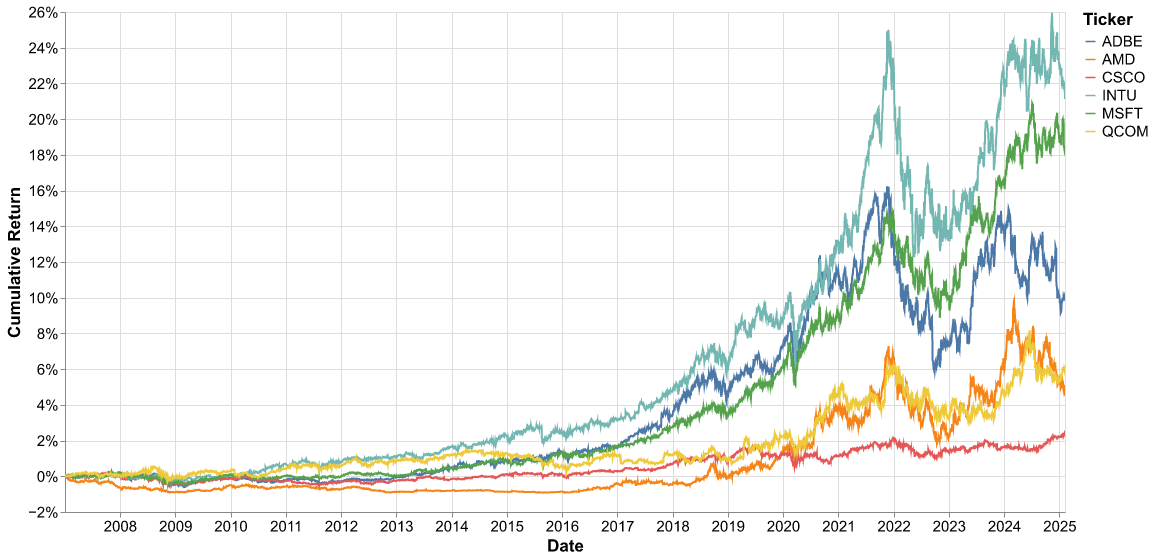
\includegraphics[width=0.9\linewidth]{plots/cumulative_returns.png}
	\caption{Cumulative Returns for the sample securities}
	\label{fig:cum_returns}
\end{figure}
Figure (\ref{fig:cum_returns}) shows the cumulative returns for the securities in our sample: ADBE, AMD, MSFT, and QCOM (as AAPL and NVDA are large cap stocks with very large momentum, visualizations for them are presented in the appendix). As we can see, within a 17-year period, INTU received the greatest cumulative return of 21.12\%; MSFT has a close second with a cumulative return of 18.25\%; from there, the rest are far behind. As expected, this is inconsistent with the descriptive statistics we have provided earlier. Cumulative returns ignore risk and measure the total percentage return, whereas metrics such as the standard deviation, $\hat{\sigma}_x$, and kurtosis, $\hat{K}(x)$, account for risk. Despite AMD and ADBE having larger returns on a risk-adjusted basis, INTU and MSFT seems to perform better than their peers. To analyze this further, we need to employ more time series techniques to capture volatility.
\begin{figure}[h]
	\centering
	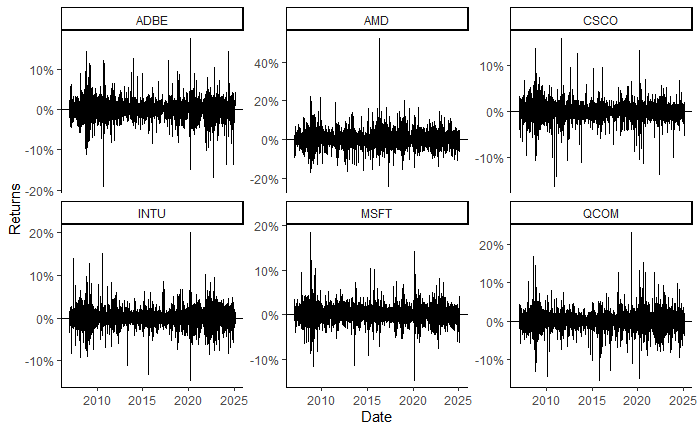
\includegraphics[width=1\linewidth]{plots/daily_returns_alt.png}
	\caption{Daily log returns for sample securities}
	\label{fig:daily_log_returns}
\end{figure}
The idea of studying volatility is that the returns of our asset $\lbrace r_t\rbrace$ have a serial correlation, or it may merely be stationary. Figure (\ref{fig:daily_log_returns}) shows the daily log returns of our sample securities. There appears to be a high degree of stationary among our sample securities, each with different clusters of volatility around specific information shows (e.g., MSFT was the most volatile during the 2008 Financial Crisis; however, ADBE was the most volatile during the 2020 Pandemic). Since log returns often appear random and volatile, it is difficult to distinguish between stationary and non-stationary processes visually. We also have the concept of drift and a change in variance. To deal with this problem, we implement the an Autocorrelation Function (ACF).

The Autocorrelation Function (ACF) measures the correlation between a time series and its own past values at different lags. It helps identify patterns, dependencies, and stationarity in time series data. When considering a weakly stationary return series, $r_t$, the linear dependence between $r_t$ and past values of $t_{t-i}$ is called the lag-$\ell$ autocorrelation of $r_t$, denoted by the following:
\begin{equation}
	\hat{\rho}_\ell=\frac{\sum_{t=\ell+1}^{T}\left(r_t-\bar{r}\right)\left(r_{t-\ell}-\bar{r}\right)}{\sum_{t=1}^{T}\left(r_t-\bar{r}\right)^2},\quad 0\leq\ell<T-1
\end{equation}
For testing several autocorrelations jointly, we have the Ljung and Box test, denoted by,
\begin{equation}
	\mathcal{Q}(m)=T(T+2)\sum_{\ell=1}^{m}\frac{\hat{\rho}_\ell^2}{T-\ell}
\end{equation}
The hypothesis test for Ljung and Box is established as follows:
\[
\begin{aligned}
	H_0&:\rho_1=\cdots=\rho_m=0\\
	H_a&:\rho_i\neq 0
\end{aligned}
\]
for some $i\in\lbrace1,\ldots,m\rbrace$. We assume that $\lbrace r_t\rbrace$ is an iid sequence and $\mathcal{Q}^*(m)$ is a chi-squared random variable, $\mathcal{X}$, with $m$ degrees of freedom. The decision rule is to reject $H_0$ if $\mathcal{Q}(m)>\mathcal{X}^2_\alpha$, where $\mathcal{X}^2_\alpha$ denotes the $100\left(1-\alpha\right)$th percentile of a chi-squared distribution. 

Figure (\ref{fig:acf_plot}) shows the sample autocorrelation functions of the monthly log returns from January 2007 to November 2025. We have used a maximum of 20 lags. In each plot, two horizontal dashed lines denote two standard error limits of ACF. The sample ACFs or the MSFT plot are very close to each other, and they suggest that the serial correlations of monthly MSFT log stock returns are very small, if any. The sample ACFs are all within their two standard error limits, indicating that they are not significantly different from zero at the 5\% level.

\begin{figure}[h]
	\centering
	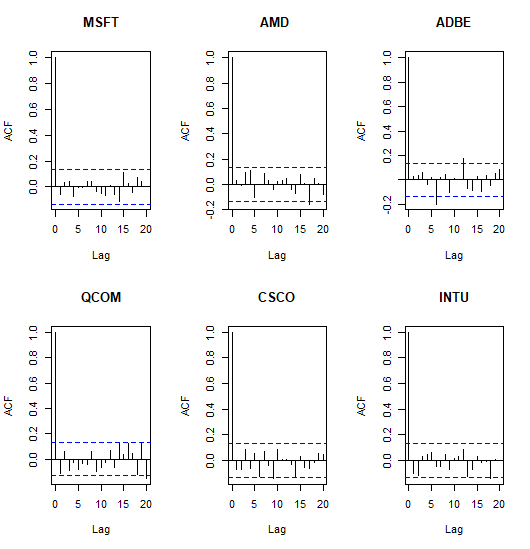
\includegraphics[width=0.7\linewidth]{plots/acf_monthly_returns.png}
	\caption{ACF Plots of log monthly returns of sample securities}
	\label{fig:acf_plot}
\end{figure}

Regarding the log monthly returns for the other securities in our sample, we find there is at least one lag that determines a significant serial correlation with previous returns. For QCOM, this occurs at lag 17; for ADBE, it's lags 6 and 12; for QCOM, it's lags 19 and 20; for CSCO, it's lags 9 and 14; for INTU, it's lag 18; and for NVDA, it's lag 4. From looking at the ACF plots, it would appear that these lags barely reach the rejection threshold of 2 times the standard error. However, we can perform the Ljung-Box statistic determine if there are some significant serial correlations at the 5\% level for all return series. The Ljung-Box statistic gives us the following:
\begin{itemize}
	\item AMD: $\mathcal{Q}(17)=19.044$, $p-$value=0.326
	\item ADBE: $\mathcal{Q}(6)=10.404$, $p-$value=0.1086; $\mathcal{Q}(12)=20.765$, $p-$value=0.05393
	\item QCOM: $\mathcal{Q}(19)=29.27$, $p-$value=0.06185; $\mathcal{Q}(20)=34.939$, $p-$value=0.02043
	\item CSCO: $\mathcal{Q}(9)=14.675$, $p-$value=0.1003; $\mathcal{Q}(14)=20.773$, $p-$value=0.1076
	\item INTU: $\mathcal{Q}(9)=20.678$, $p-$value=0.296;
	\item NVDA: $\mathcal{Q}(4)=10.826$, $p-$value=0.028;
\end{itemize}
As we can see from the test statistics and the $p$-values, the only securities with a significant serial correlation with monthly log returns are QCOM and NVDA. What we can interpret from this data, at least for long monthly returns, is that there is no significant serial correlation. It may be worth using a more frequent observation series, such as daily.

We have also looked at the Partial Autocorrelation Function (PACF) of the log monthly returns. The PACF is used to directly measure the relationship between a time series and its past values at different lags while removing the influence of the intermediate lags. Unlike the ACF, which includes direct and indirect correlations, the PACF isolates the pure effect of each lag on the present value.
\begin{figure}[h]
	\centering
	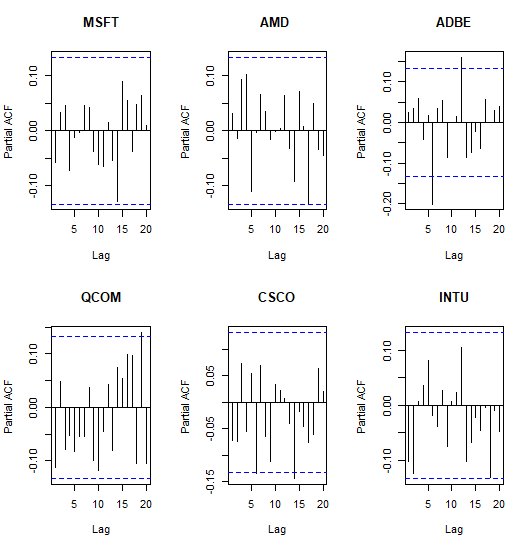
\includegraphics[height=0.8\linewidth]{plots/pacf_monthly_returns.png}
	\caption{PACF Plots of log monthly returns of sample securities}
	\label{fig:pacf_plot}
\end{figure}
Figure (\ref{fig:pacf_plot})shows the PACF for the log monthly returns for our sample securities. We have used a maximum of 20 lags. After accounting for intermediate lags, each bar in the PACF plot represents the correlation between the time series and its lagged version. The dashed lines represent the 95\% confidence interval. Any bar extending beyond these lines is statistically significant. ADBE and CSCO all appear to have significant lags.

ADBE have significant lags at month 6 and month 12; meaning the returns 6 and 12 months have a direct influence on the current month returns. This suggest that monthly log returns of ADBE may have some seasonal dependency. With CSCO, we have significant lags at month 6 and 14, suggesting the log monthly returns from 6 and 14 months ago have a direct influence on the log monthly returns in the current month.
\subsection*{Unit-root and Seasonality}
To test whether the log price $p_t$ of an asset follows a random walk, we would need to employ the following models
\begin{equation}
	\begin{aligned}
		p_t&=\phi_1p_{t-1}+\epsilon_t\\
		p_t&=\phi_0+\phi_1p_{t-1}+\epsilon_t
	\end{aligned}
\end{equation}
where $\epsilon_t$ denotes the error term. We need to consider the null hypothesis
\begin{equation}
	\begin{aligned}
		H_0:\phi_1=1\\
		H_a:\phi_1<1.
	\end{aligned}
\end{equation}
Where the test statistic is
\begin{equation}
	\hat{\phi}_1=\frac{\sum_{t=1}^{T}p_{t-1}p_t}{\sum_{t=1}^{T}p^{2}_{t-1}},\quad\hat{\sigma}^2_\epsilon=\frac{\sum_{t=1}^{T}(p_t-\hat{\phi}_1p_{t-1})^2}{T-1}
\end{equation}
where $p_0=0$ and $T$ is the sample size. If the null hypothesis shows that $\phi_1=1$, we fail to reject the null hypothesis, which say that the time series has a Unit Root. Otherwise, we can reject the null hypothesis and consider the time series as stationary. We perform this hypothesis test with a technique commonly referred to as the augmented Dickey-Fuller (ADF) unit-root test.

\begin{figure}[h]
	\centering
	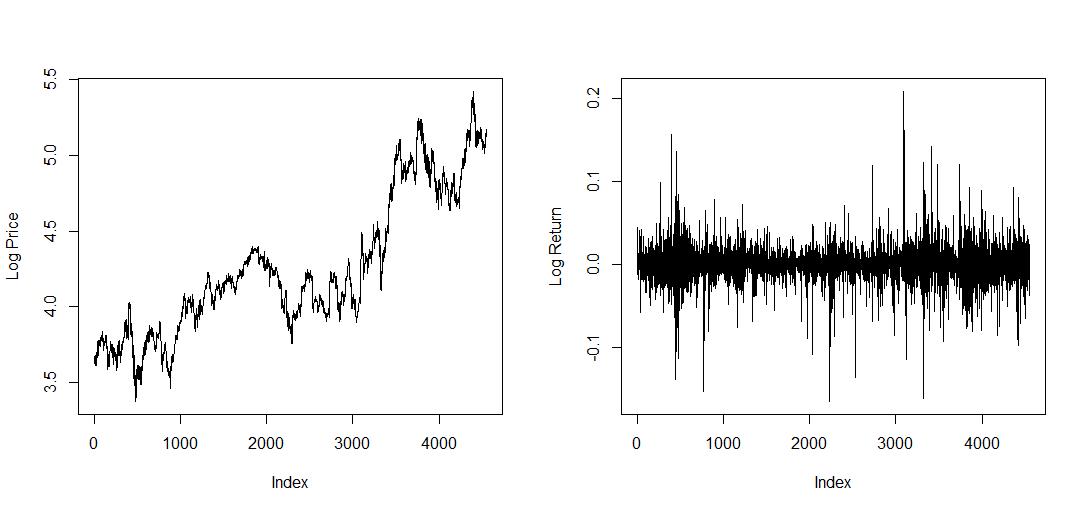
\includegraphics[width=0.9\linewidth]{plots/qcom_log_price_return.png}
	\caption{Time Series of QCOM Log Prices and Returns }
	\label{fig:qcom_log_price}
\end{figure}

Figure (\ref{fig:qcom_log_price}) shows the log returns and prices of the QCOM. We took the log transformation for two reasons. First, it is used to handle the exponential growth of the series, which the plot on the left confirms that the growth is linear on a log scale. Second, the transformation is used to stablize the variability of the series. With these adjustments in mind, we can see that the log price exhibit an upward trend. On the other hand, the variability changes throughout the time series when it comes to the log returns. Despite this, the log of the log returns is clearly stationary. We implemented the augmented Dickey-Fuller test on both the log prices and returns.
\begin{table}[ht]
	\centering
	\caption{Augmented Dick-Fuller Test for QCOM}
	\begin{tabular}[t]{lcccc}
		\toprule
		Time Series &Lag order& t-statistic & $p$-value & Outcome  \\
		\midrule
		Log Prices & 16 & -3.051 & 0.1333 & Unit-Root  \\				
		Log Returns & 16 & -16.254 & 0.01 & Stationary  \\				
		\bottomrule
	\end{tabular}\label{tab:adftest}
\end{table}
Table (\ref{tab:adftest}) shows the output of the augmented Dickey-Fuller test for the log prices and returns of QCOM. As we can see our suspicions were correct; we fail to reject the null-hypothesis for the log prices, but reject the null-hypothesis for the log returns. As such, the log returns are stationary, while the log prices exhibit unit-root.

We establish the time series' seasonality by examining the log prices' sample ACF. Figure (\ref{fig:qcom_acf_plots}) shows the ACF plots of QCOM with varying differencing and seasonality implementations. We have used a maximum lag of 100, with the time and seasonal differencing of once every 30 lags. The autocorrelation plot on the top right contains a very high and slow decay, starting from 1 at lag 0, which decreases gradually. This is typical of a non-stationary time series, where the values of the sample ACF are highly dependent on their past, such as a random walk.

\begin{figure}[h]
	\centering
	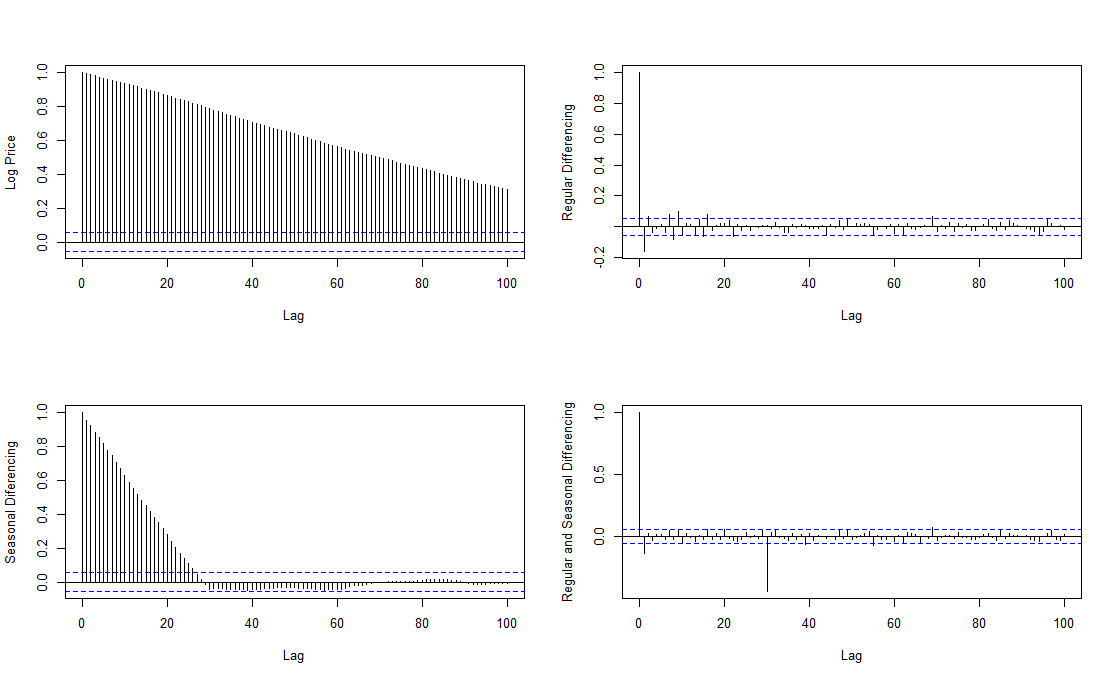
\includegraphics[width=1\linewidth]{plots/acf_plot_time_series.png}
	\caption{ACF Plot of QCOM }
	\label{fig:qcom_acf_plots}
\end{figure}

The plot on the top right shows the ACF of the First differenced log prices of the daily log prices. We can see a sharp drop in the autocorrelation at lag 1, where the other lags are within the confidence bounds. The first differencing has successfully removed the trend, producing a series that now looks more like white noise. 

On that bottom left plot, we have the ACF of the seasonal differencing, with a strong autocorrelation at lower lags, which slowly decreases to zero around lag 30. The differencing involves the following formula

\begin{equation}
	\Delta_{30}(\Delta x_t)=(1-B^{30})\Delta x_t=\Delta x_t-\Delta x_{t-30}
\end{equation}

After lag 30, the values fluctuate randomly around zero. This suggests that seasonal differencing alone removes the long-run periodicity but not the trend of the time series. In other words, seasonal differencing alone is not enough to transform the plot into a stationary time series.

The final plot on the bottom right shows the ACF after regular and seasonal differencing. The pattern shows that almost all autocorrelations are within the confidence bands, except for a substantial spike at lag one and lag 30, which suggest a seasonal lag. As we can see, combining regular and seasonal differencing yields a stationary series, and the residual autocorrelations are minimal. These transformations show that the plots on the bottom left and right show a stationary transformation. Fitting an ARIMA model would involve implementing either regular differencing or both regular and seasonal differencing.

\section*{ARIMA Model}

The goal of this section is to fit log prices and log returns into an autoregressive (AR), moving average (MA) or some combination of the two (ARMA, ARIMA). 	Figure (\ref{fig:acf_pacf_log_price_returns}) shows the ACF for the log prices (a), PACF of the log prices (b), ACF for the log returns (c) and the PACF for the log returns (d). For AR models, we would expect the ACF to show a gradual decay where the tail cuts off at some point, where the PACF would sharply cut off at lag $p$, then drops to approximately zero. For MA models, we would expect the opposite, where the ACF significantly cuts off at lag $q$ (then drops off to near zero) and the ACF would gradually decay.

\begin{figure}[h]
	\centering
	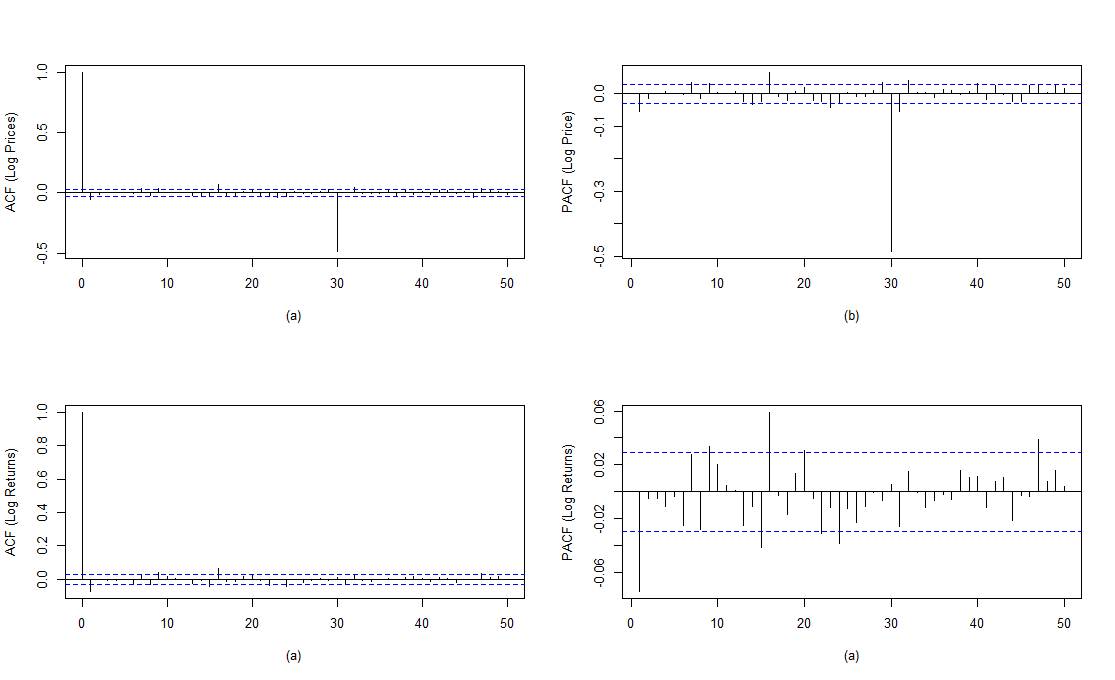
\includegraphics[width=1\linewidth]{plots/acf_pacf_log_price_returns.png}
	\caption{ACF and PACF for the log returns/prices of QCOM}
	\label{fig:acf_pacf_log_price_returns}
\end{figure}

\subsection*{}
\end{document}